This section describes the purpose, intended use, and target users of the Agrihome product. Agrihome is a smart indoor plant monitoring and early disease detection system designed to help users observe plant health before visible damage becomes severe. The system combines image capture, environmental sensing, backend analysis, and a user-facing dashboard to provide health insights, warnings, and historical tracking for home and small-scale growers.

\subsection{Purpose and Use}
Agrihome is intended to support plant owners by continuously monitoring plant condition and identifying potential health problems as early as possible. The product focuses on indoor use and is especially suited for crops or household plants that benefit from regular observation, such as tomatoes and other small garden plants.

The system is designed to capture plant images from one or more cameras and collect supporting environmental data such as temperature, humidity, soil moisture, and light level when sensors are available. Captured data is analyzed by the software system to classify the plant as healthy or potentially unhealthy, and to identify likely issues such as leaf disease symptoms or environmental stress. The result is then presented to the user through a dashboard or application interface.

In normal use, a user places the plant within the monitoring area, powers the system, and connects to the dashboard. Agrihome then performs scheduled monitoring without requiring the user to manually inspect the plant each time. When the system detects abnormal plant conditions, it provides a warning and a short explanation so the user can take action earlier. The product is intended to reduce guesswork, improve response time to plant problems, and make plant care easier for non-expert users.

Agrihome is not intended to physically treat the plant, apply chemicals, or replace professional agricultural diagnosis. Instead, it acts as an intelligent monitoring and decision-support tool for plant care in home or small-scale environments.

\subsection{Intended Audience}
The primary intended audience for Agrihome includes home gardeners, apartment growers, student researchers, and hobbyists who want a practical way to monitor plant health with less manual effort. The product is especially useful for users who may not have advanced agricultural knowledge but still want timely feedback about plant condition.

A secondary audience includes academic teams, senior design evaluators, and small greenhouse or controlled-environment users who may use the system as a prototype platform for plant monitoring research and experimentation.

If made commercially available, Agrihome would be most attractive to consumers interested in smart gardening, indoor growing, and automated plant care support. The product is designed as a standalone monitoring system, but it could also serve as a subsystem within a larger smart agriculture or smart home platform.

\begin{figure}[h!]
\centering
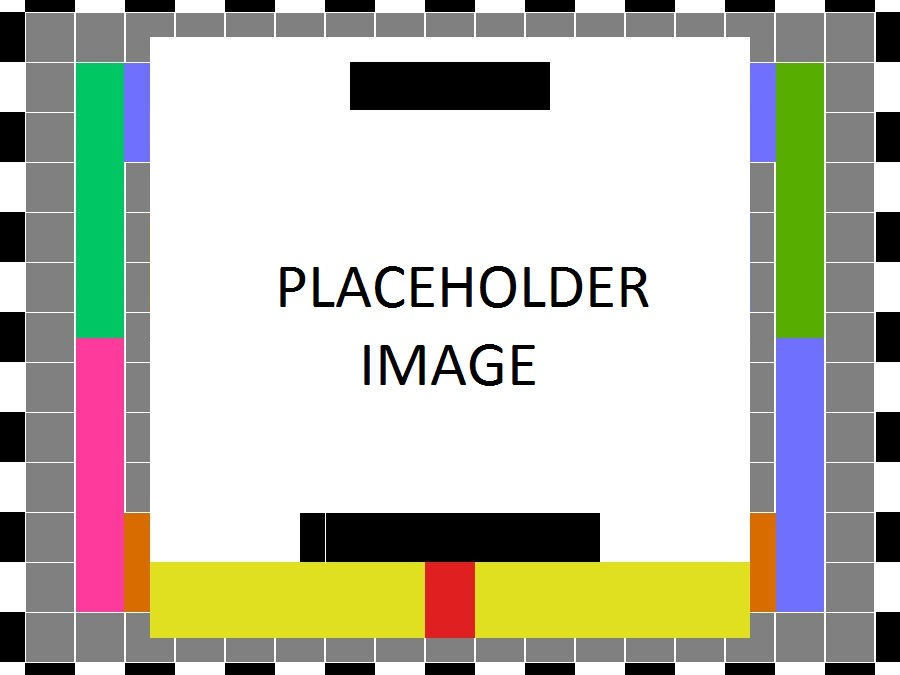
\includegraphics[width=0.60\textwidth]{images/test_image}
\caption{Agrihome conceptual overview}  \end{figure}
